\chapter{Search Trees}
\label{ch:search-trees}

\section{How to Find a Folder}

Suppose you have a bunch of file folders (physical ones, those
manilla-colored things, not folders on the computer system). Each
folder contains some documents and is identified by a number on its
filing tab. Every now and then someone gives you an identifying
number and asks you to retrieve the corresponding folder. How much
work is that going to be?

It depends on the number of file folders and the care you take in
organizing them. If you have only a few folders, it doesn't matter
much. You can just scatter them around on the desktop, and when
you're asked to get one, look around until you find it. It might be
in the first folder you pick up, or the second, and the worst that
can happen is that you will have to look at all of the folders
before you find the one you want. Since there aren't very many, it
won't take long.

That's fine when there are only a few folders, but what if there
were hundreds? Then, the frustration in finding the right folder
might motivate you to rethink the arrangement. Scattering the
folders around the desktop would be an unattractive way to keep
track of them. You might go out and buy a four-drawer filing cabinet
and arrange the folders in the cabinet in order by their identifying
numbers. When somebody asks you for a particular folder, you quickly
locate the folder by relying on the numbering. Much better, eh?

How much better? Say you have a thousand folders and you were using the
old desktop method. Sometimes you would find it on the first go,
sometimes the second, sometimes the thousandth. Because the folders
are scattered on the desktop at random, no folder is more likely to
be the one you're looking for than any other folder, so the average
search time would be the average of the numbers 1, 2,\dots 1,000,
which is about 500.

Now, how about the filing-cabinet method? The time it takes you here
depends on how much you take advantage of the numbering, but it
turns out that the typical search time will be much improved over
the desktop method.

You could proceed by looking at
the identifying number and comparing it to the number on the middle
file in your four-drawer cabinet.
If the number on the folder you're looking for is bigger than the first one in
the middle file drawer, then you know to look in the bottom half of the
file drawers. If it's smaller, you look in the top half.
That is, you've narrowed down the search to two of the four file drawers.

Then, you could do the same thing again to narrow it down to one file drawer,
and after that, look at a folder near the middle of the file drawer
to figure out whether the one you're looking for is in the front half
of the drawer or the back half.
At each stage, you eliminate half of the folders.
When you started, the folder you're looking for might have been any
of the 1,000 folders. After the first step, you can limit your search
to 500 folders. After the second step, 250 folders, and so on,
halving the number of candidates at each stage until you finally
narrow it down to one folder.

Of course, you might have found it somewhere along the way,
but the worst that can happen is that you don't find it until you
narrow it down to one folder. That takes ten steps, worst case, so
the average case must be at least that good, which
fifty times better than the 500-step average required in the desktop method.

Good as that sounds, it gets even better. If you have 10,000 folders,
instead of just 100, the first go knocks it down to 5,000 folders,
then 2,500, and so on down to a single folder in fourteen steps, max,
for the filing cabinet method, which is hundreds of times faster
than the 5,000-step average for the desktop method.
If you have a million
folders, the improvement is even more dramatic. With a million
folders, the filing cabinet method has a twenty-five-thousand-fold
advantage over the desktop method. It gets better and better, the
more folders you have. Of course, you will have to buy more filing
cabinets, but regardless of how many filing cabinets you have,
you can halve the search space at every stage.

\section{The Filing Cabinet Advantage}

Let's work out a formula for the filing-cabinet advantage. If you
have $n$ folders, the most steps you have to make in your search is
the number of times you have to successively halve $n$ to get down
to one. That number is the base-two logarithm of $n$. Actually,
the logarithm is not an integer, it's the next integer up, so
round up to the next integer.
The notation $\lceil x \rceil$ means the smallest integer that is
$x$ or bigger.
For example $\lceil 3.5 \rceil$ is 4.

Here are the formulas for the typical number of steps in the two
methods: desktop versus filing cabinet, as functions of the number
of folders.

\begin{tabular}{ll}
D(n) = $\lceil n/2 \rceil$      & \emph{desktop method} \\
C(n) = $\lceil log_2(n) \rceil$ & \emph{filing cabinet method} \\
\end{tabular}

The ratio $D(n)/C(n)$ expresses the advantage of the filing-cabinet
method over the desktop method. As the examples indicated, it gets
better and better as $n$, the number of folders, gets larger. For a
billion folders, there is more than a ten-million-fold advantage.
Plus, the desktop would be long buried by that time,
and the folders would be scattered all over the office building.

\section{The New-File Problem}

\label{binary-search}
The filing-cabinet method performs an algorithm known as a
``binary search''.
It's a simple idea, and
probably one that almost anyone would think of, faced with the
problem of organizing a large number of folders for retrieval
purposes. It works amazingly well, as long as the number
of folders doesn't change very often.

However, when a new folder needs to be added to the
collection, it can be a problem. The problem usually doesn't come up
on the first few new folders. For those, there will be room to
squeeze them into the drawers where they belong. The problem comes
up when the number of folders keeps growing. Eventually, there is no
room left in the drawer where a new folder belongs, so some of the
folders in that drawer have to be moved down to another drawer to
make room. What's worse, the next drawer may also be full. The
problem can cascade further and further along. With a whole office
building filled with cabinets for billions of folders, putting in
one new folder can call for a lot of heavy lifting.

In fact, with an office building filled with cabinets, it will be
advantageous to keep the folders in as few cabinets as possible. If
they were scattered out, and many cabinets were nearly empty, there
could be a lot of walking involved to find the appropriate cabinet.

In other words, to keep down the walking, folders must be kept in
the smallest number of drawers possible. This means that the drawers
involved are almost always full, and whenever a new folder comes in,
a bunch of folders have to be moved around to accommodate the new
one.

How much moving around? As in the desktop method, it depends on
where the new folder goes. If it goes at the end, no problem. Just
put it at the end of the last non-empty drawer. But, if it goes at
the beginning, all of the folders must be moved down one slot to
accommodate the new one. Bummer!

On the average, just as with finding folders using the desktop
method, about half of the folders must be moved to accommodate a new
folder. Something similar happens if a folder needs to be discarded.
Again, on the average, about half of the folders must be moved to
keep the folders compressed into the smallest number of drawers.

\section{The AVL Solution}

In a computer, the filing-cabinet method is normally implemented
using an array to store the folders. The identifying numbers on the
folders are arranged in order in the array, and to find a particular
identifying number, the software looks first at the middle element
of the array, then at the middle element of the narrowed ranged
resulting from the first comparison of identifying numbers, and so
on. That is, a binary search is performed in the array.

When a new folder comes in, it must be inserted in the
place required by its identifying number to keep the numbers
in order. So, all of the elements beyond that point
must be moved down to make room. This can be time-consuming if there
are, say, billions of folders in the array.

The same thing happens in deleting a folder from the array. All the
folders beyond the point of deletion must be moved up to eliminate
the gap. In either case, the number of array elements to be moved
is, on the average, about half of the number of folders in the array.
That's not good, and it's not an easy problem to fix.
In fact, it can't be fixed with array-based methods.

In the 1960s (ancient history in the computing business),
two Russian mathematicians, Adelson-Velskii and Landis,
figured out a way to store folders in a tree structure so that
finding a folder, adding a new folder, and removing a folder all
require only about $log(n)$ steps, where $n$ is the number
of folders stored in the tree. The structure these mathematicians
invented, together with their insertion and deletion methods, is
known as the AVL tree. \label{AVL-tree}

The simple part of the Adelson-Velskii/Landis solution is to store
the folders in a tree that facilitates binary search. Except for
leaf-nodes, each node in the tree stores a folder and has a left
subtree and a right subtree. (Leaf nodes just mark the boundaries of
the tree. They don't store folders, and they don't have subtrees.)
All of the folders in the left subtree have identifying numbers that
are smaller than that of the folder in the root node (that is,
the one you start with), and all of
the folders in the right subtree have identifying numbers that are larger.
To find a folder, look at the root. If the folder stored at
the root has the identifying number you're looking for, deliver that folder.
If not, look at the left subtree if the sought-for identifying number
is smaller than the one in the root, and look in the right subtree
if it is larger.

If a folder with the identifying number you're looking for is in the tree,
it will be found.
Otherwise, the search will arrive at a leaf-node,
indicating that the required folder is not in the tree.

That's the simple part. The hard part has to do with insertion and
deletion. The number of steps in the search depends on where the
folder occurs in the tree, but at worst, the number of steps cannot
exceed the number of levels in the tree. Nodes in a tree have
subtrees, and the subtrees have subtrees, and so on.
Eventually, the desired folder is encountered, or a leaf is
encountered, and the search cannot continue. The maximum number of
steps in this search, for all possible search paths in the tree, is
known as the $\emph{height}$ of the tree.
AVL trees maintain a balance among subtree heights, at all levels,
as nodes are inserted and deleted.
By maintaining balance, the AVL tree
preserves a high ratio between number of folders it contains and the
height of the tree.

In fact, the height of an AVL tree is approximately the base-2
logarithm of the number of folders it contains. That means every
search will terminate within $log_2(n)$ steps, where $n$ is the
number of folders stored in the tree.

If you want to get a feeling for just how ingenious the AVL
solution is, try to find a way to insert folders into a
tree that maintains order (left subtrees have folders with smaller
identifying numbers, right subtrees larger) and balance (left
subtrees have about the same number of nodes as right subtrees, at
all levels). To match the effectiveness of AVL trees, your method
will have to be able to insert or delete a folder in about
$log(n)$ steps, where $n$ is the number of folders stored
in the tree.
After a few hours work, you'll begin to appreciate
the contribution that Adelson-Velskii and Landis made to the technology for
maintaining large data bases.

\section{Search Trees and Occurrence of Keys}

It's a long road from here to the complete AVL solution.
As usual, the road starts with formulas and equations that make the ideas
amenable to mathematical reasoning.
The first step is to define a formal representation of a tree.

To avoid unnecessary details, the definition
does not specify the kind of data associated with nodes.
They may contain any kind of data.
We assume that each node is identified by a numeric key,
which is the basis for locating the node.
We are going to assume that keys are natural numbers,
but any set with an ordering among its elements could serve
as the domain of the keys.

\label{leaf-node}
Each node in the tree is either a ``leaf node'', represented by ``nil'',
\label{interior-node}
or an ``interior node'', represented by a list of four elements:
key (a number), data (of any kind), left subtree, and right subtree.
\label{root-node}
The ``root node'' is the one that is not preceded by any other node.
In the diagram, it's the node at the top.
In a formula, it's the entire formula.
The key of the root node is the first element of the list that represents the tree,
and the data associated with the root is the second element.

We will be using ``binary trees'', which are trees
in which each node has no more than two subtrees.
We only need two subtrees to be able to use binary search
to find items in the tree.

Figure \ref{fig:searchtree-diagram} shows a formula
for a search tree in which the data are strings.
The algebraic formula represents the tree in the diagram.
We will rely extensively on diagrams to
illustrate ideas expressed algebraically in terms of formulas.
You will need to develop an ability to see the connection
and convert freely between diagrams and formulas.

\begin{figure}
\begin{center}
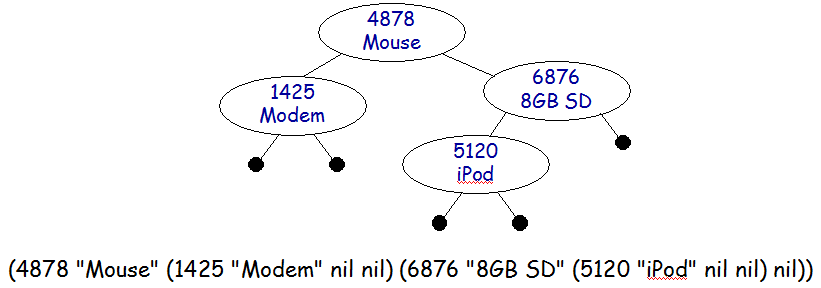
\includegraphics[scale=0.5]{images/searchtree.png}
\end{center}
\caption{Search Tree Diagram and Corresponding Formula}
\label{fig:searchtree-diagram}
\end{figure}

\label{empty-tree}
We use nil to represent the empty tree.
For non-empty trees, we use
four-element lists in which the key and data at
the root are the first two elements and the left
and right subtrees are the last two elements.
\label{subtree}
A ``subtree'' is any part of a tree beginning with a node
other than the root
and continuing all the way from that node to the leaves.
A key occurs in a search tree if it is the key at the root
or if it occurs in either the left or right subtree.

\label{height}
The height of an empty tree is zero, by default.
The height of a non-empty tree is one more than the
larger of the heights of its left and right subtrees.
The size of a search tree is the number of keys in the tree.

Figure \ref{fig:tree-functions} makes these ideas precise
by providing formal definitions.

\begin{figure}
\begin{center}
\begin{Verbatim}
(defun key (s) (first s))          ; key at root
(defun dat (s) (second s))         ; data at root
(defun lft (s) (third s))          ; left subtree
(defun rgt (s) (fourth s))         ; right subtree
(defun emptyp (s) (not (consp s))) ; empty tree?
(defun height (s)                  ; tree height
  (if (emptyp s)
      0                                               ; ht0
      (+ 1 (max (height (lft s)) (height (rgt s)))))) ; ht1
(defun size (s)                    ; number of keys
  (if (emptyp s)
      0                                     ; sz0
      (+ 1 (size (lft s)) (size (rgt s))))) ; sz1
(defun n-element-list (n xs)
  (if (zp n)
      (equal xs nil)
      (and (consp xs) (n-element-list (- n 1) (rest xs)))))
(defun treep (s)                  ; search tree?
  (or (emptyp s)
      (and (n-element-list 4 s) (natp (key s))
           (treep (lft s)) (treep (rgt s)))))
(defun subp (r s)                ; r subtree of s?
  (and (treep r) (treep s) (not (emptyp s))
       (or  (equal r (lft s)) (subp r (lft s))
            (equal r (rgt s)) (subp r (rgt s)))))
(defun keyp (k s)                ; key k occurs in s?
  (and (not (emptyp s))
       (or (= k (key s)) (keyp k (lft s)) (keyp k (rgt s)))))
\end{Verbatim}
\end{center}
\caption{Search Tree Functions and Predicates}
\label{fig:tree-functions}
\end{figure}

The only tree of height zero is the empty tree because
the height of a non-empty tree is one more than the maximum
of two other numbers, which makes it at least one.
Furthermore, the height of a subtree is strictly less than the height of the tree.
Theorems \{\emph{ht-emp}\} and \{\emph{subtree height}\}
are formal statements of these facts.

Theorem \{\emph{ht-emp}\} ((height $s$) = 0) = (emptyp $s$)

Theorem \{\emph{ht} $<$\}. (subp $r$ $s$) $\rightarrow$ ((height $r$) $<$ (height $s$))

Proof of \{\emph{ht} $<$\}: induction on the height of the tree

Base case: (height $s$) = 0, so (emptyp $s$) = true \{\emph{ht-emp}\}

%\begin{center}
\begin{tabular}{rll}
     & (subp $r$ $s$) $\rightarrow$ \dots              & \\
 $=$ & (and (treep $r$) (treep $s$) (not (emptyp $s$))) \dots)  $\rightarrow$ \dots & \{\emph{emptyp}\} \\
 $=$ & (and true true (not true)) $\rightarrow$ \dots  & \{\emph{assumption}\} \\
 $=$ & (and true true nil) $\rightarrow$ \dots         & \{$\neg$ \emph{truth table}\} \\
 $=$ & nil $\rightarrow$ \dots                         & \{$\wedge$ \emph{truth table}\} \\
 $=$ & true                                            & \{$\rightarrow$ \emph{truth table}\} \\
\end{tabular}
%\end{center}

In the inductive case, (height $s$) $>$ 0.
We conclude that (emptyp $s$) is false
as a consequence of the \{\emph{ht-emp}\} theorem.
Therefore, the definition of (subp $r$ $s$) reduces to
($r$ = (lft $s$)) $\vee$ (subp $r$ (lft $s$)) $\vee$
($r$ = (rgt $s$)) $\vee$ (subp $r$ (rgt $s$)).
So, we can prove the inductive case by deriving it from
each of operands of this $\vee$-formula, independently (\{$\vee$ \emph{elimination}\}).
We refer to these four cases as ``inductive case 1'', inductive case 2'', etc.
The following proof deals with the inductive case 2: (subp $r$ (lft $s$)).
Proofs of the other inductive cases are similar.

Inductive case 2: (subp $r$ (lft $s$)) is true

%\begin{center}
\begin{tabular}{rll}
       & (height $s$)                                    & \\
 $=$   & 1 + (max (height (lft $s$)) (height (rgt $s$))) & \{\emph{ht1}\} \\
 $\ge$ & 1 + (height (lft $s$))                          & \{\emph{algebra}\} \\
 $>$   & 1 + (height $r$)                                & \{\emph{induction hypothesis}\} \\
 $>$   & (height $r$)                                    & \{\emph{algebra}\} \\
\end{tabular}
%\end{center}

\section{Ordered Search Trees}

A search tree is ``ordered'' if the key in each non-leaf node is
greater than all the keys that occur in the left subtree of the node
and is less than all the keys that occur in the right subtree. A
leaf is ordered by default.
The following equations of predicate calculus define
``ordp'':
(ordp $s$) is true if $s$ is ordered and false otherwise.

\begin{center}
\begin{tabular}{lll}
(ordp nil) = & true & \{\emph{ord0}\} \\
(ordp $s$) = & ($\forall x$.((keyp $x$ (lft $s$)) $\rightarrow$ $x$ < (key $s$))) $\wedge$ (ordp (lft $s$)) $\wedge$ & \{\emph{ord1}\} \\
             & ($\forall y$.((keyp $y$ (rgt $s$)) $\rightarrow$ $y$ > (key $s$))) $\wedge$ (ordp (rgt $s$))          & \\
\end{tabular}
\end{center}

From the definition of ordp, it's not a big step to
guess that an ordered search tree cannot contain duplicate keys.
However, saying exactly what that means turns out to be tricky.
One approach is to prove that if a key occurs at the root,
then it doesn't reside in either subtree, and if it occurs
in one subtree, then it doesn't occur in the other subtree or at the root.

%\begin{tabular}{ll}
Theorem \{\emph{keys unique}\}. (ordp $s$) $\rightarrow$ \\
((($k$ = (key $s$)) $\rightarrow$ ((not(keyp $k$ (lft $s$))) $\wedge$ (not(keyp $k$ (rgt $s$))))) $\wedge$ \\
(((keyp (lft $s$))) $\rightarrow$ (($k$ $\ne$(key $s$)) $\wedge$ (not(keyp $k$ (rgt $s$))))) $\wedge$ \\
(((keyp (rgt $s$))) $\rightarrow$ (($k$ $\ne$(key $s$)) $\wedge$ (not(keyp $k$ (lft $s$)))))) \\
%\end{tabular}

Stating this theorem about as complicated as proving it.
The proof simply applies the definition of ordp judiciously in each circumstance.
For example, if $k$ = (key $s$), then (keyp $k$ (lft $s$)) must be false
because if (keyp $k$ (lft $s$)) were true, then $k$ $<$ (key $s$),
according to the definition of ordp. That is inconsistent with  $k$ = (key $s$),
so (keyp $k$ (lft $s$)) must be false (\{\emph{reductio ad absurdum}\}).
By a similar argument, (keyp $k$ (lft $s$)) also must be false.
So, the first operand of the $\wedge$ formula of the theorem is true.
Proving that the other two operands are also true can be done
with similar reasoning from the definition of ordp.
Since each operand of the $\wedge$ formula is true when the hypothesis
of the implication (ordp $s$) is true,
the implication formula that comprises the theorem is true
(\{$\wedge$ implication\}, page \pageref{and-implication})

\begin{ExerciseList}
\Exercise Prove that
(ordp $s$) $\rightarrow$ (((keyp $k$ (lft $s$))) $\rightarrow$ (($k$ $\ne$(key $s$)) $\wedge$ (not (keyp $k$ (rgt $s$)))))
is true.

\Exercise Prove that
(ordp $s$) $\rightarrow$ (((keyp $k$ (rgt $s$))) $\rightarrow$ (($k$ $\ne$(key $s$)) $\wedge$ (not (keyp $k$ (lft $s$)))))
is true.
\end{ExerciseList}

\section{Balanced Search Trees}

Search trees must be ordered to make it convenient to find things.
However, order is not enough.
Trees must also be short, relative to the number of items in the tree.
Otherwise, order doesn't help.
It can take as long, on the average, to find an item as it would
if they were completely unorganized.
Figure \ref{fig:unbalanced-trees} (page \pageref{fig:unbalanced-trees})
compares some extreme cases to an optimally balanced case.

\begin{figure}
\begin{center}
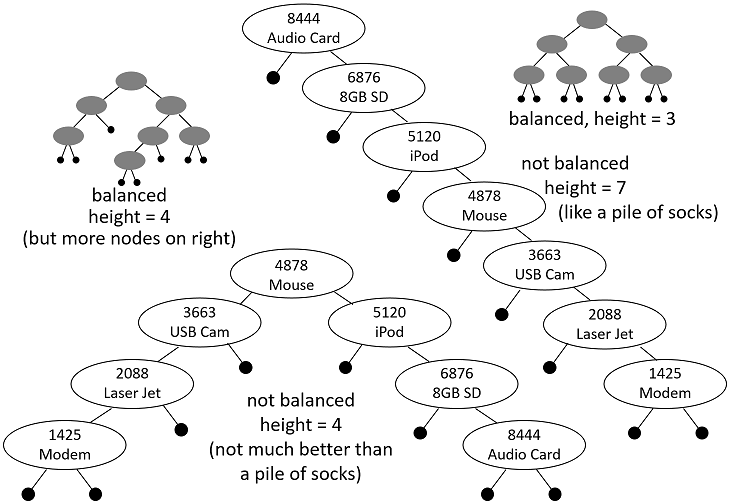
\includegraphics[scale=0.5]{images/unbalanced-trees.png}
\end{center}
\caption{Balance Shortens Trees}
\label{fig:unbalanced-trees}
\end{figure}

There are many ways to think about balance in trees.
Size balancing, for example, requires that both sides of
a tree have the same number of nodes, not only at the root,
but also for every subtree.
The tree of height seven in
Figure \ref{fig:unbalanced-trees} (page \pageref{fig:unbalanced-trees})
is unbalanced at every level (except at the bottom).
The tree of height four, on the other hand,
has the name number of nodes on the left side of the root as on the right,
but is unbalanced at the next level because
the left subtree has two nodes on the left and none on the right.
All subtrees in the tree of optimal height have
the same number of nodes on the left as on the right, so it
is size balanced. It is straightforward to demonstrate,
using inductive construction, that
the height of a size-balanced tree is $\lceil log_2 n \rceil$.
This is optimal.
The height of any tree with $n$ nodes will be at least $\lceil log_2 n \rceil$.

It turns out that, however, that we can rely on a less strict
notion of balance and still get what we need, which is logarithmic
growth in tree height.
A ``height balanced'' binary tree is


The height of a height-balanced tree is less than $1.5 \cdot log(n)$.
That makes finding things take a few more
steps than the optimal case, but the number of steps is still small.
Finding a particular key among a billion nodes
might require 45 steps instead of 30, but that's
still plenty fast compared with half a billion steps,
on the average, for unorganized data.

What we get for a few extra steps in finding things is
an astonishing improvement in the number of steps required
to insert a new node in an existing search tree.
Instead of $n/2$ steps, on the average,
for array-based methods (banks of filing cabinets),
insertion (and deletion) can be done in logarithmic time.
That is, the number of steps required to to insert or delete
a node in a search tree will be proportional to $log(n)$,
giving us the same advantage in insertion and deletion speed
that binary search provides in look-up speed.

\begin{ExerciseList}
\Exercise Prove that it is possible to put $2^n - 1$ nodes
in a binary tree of height $n$.
\end{ExerciseList}

\section{Inserting a New Item in a Search Tree}

A search tree, to be effective, must be both ordered and balanced.
Since height balancing is good enough, we won't concern ourselves
with optimal balancing. We will just make sure that both subtrees
of any node in a search tree have the same height, or that the
height of one of them is only one more than the height of the other.
The function ``balp'' expresses this notion formally.

\begin{figure}
\begin{center}
\begin{Verbatim}
(defun balp (s) ; height balanced?
  (or (emptyp s)
      (and (<= (abs (- (height (lft s)) (height (rgt s)))) 1)
           (balp (lft s) (balp (rgt s))))))
\end{Verbatim}
\end{center}
\caption{Balance Predicate}
\label{fig:balance-and-size}
\end{figure}

It is not difficult to maintaining order and balance while
inserting new items into small search trees.
To preserve order, simply find the place at a leaf node
where the new key goes.
You can do this by moving left or right down the tree according
to whether the new key is smaller or larger than the key being
considered. When you arrive at an empty tree, replace it with a
one-node tree containing the new key, its
associated data. Its subtrees will, of course, be empty.
This automatically preserves order.

If you're lucky, it may also preserve balance.
However, the replacement subtree has height 1, while the subtree it
replaced (an empty tree) had height zero. If this takes place
at a point where the tree was already a bit on the tall side,
balance can get out of whack.
If the trees goes out of balance, you have to rearrange it
to bring it back into balance, without getting keys out of order.
In small trees, it's easy to find a way to do this,
as illustrated in Aside \ref{aside:insertion-example}
(page \pageref{aside:insertion-example}).

\begin{aside}
The following example starts with a tree containing one item,
then inserts three new items, one at a time.
We use the formula (ins ($k$ $d$) $s$) to denote
the tree produced by inserting the key $k$ and associated
data $d$ into the search tree $s$.

The end result is an ordered,
balanced tree containing four items.
It will aid your understanding
of the insertion process if you draw diagrams similar to Figure
\ref{fig:unbalanced-trees} for the trees denoted by the formulas in the example.
Verify, as you go, that each tree is both ordered and height balanced.
\begin{center}
\begin{tabbing}
%
\vspace*{-1.5\topsep}
\rule{\textwidth}{0.4pt}
\vspace*{-\topsep}
%
\\
(ins \= (1125 "Modem") \\
     \> (8444 "Audio Card" nil nil)) \\
     \> $\Downarrow$ \\
(1125 "Modem" nil (8444 "Audio Card" nil nil)) \\
%
\vspace*{-1.5\topsep}
\rule{\textwidth}{0.4pt}%
\vspace*{-\topsep}
%
\\
(ins \= (4878 "Mouse") \\
     \> (1125 "Modem" nil (8444 "Audio Card" nil nil))) \\
     \> $\Downarrow$ \\
(4878 "Mouse" \= (1125 "Modem"      nil nil)  \\
              \> (8444 "Audio Card" nil nil)) \\
%
\vspace*{-1.5\topsep}
\rule{\textwidth}{0.4pt}%
\vspace*{-\topsep}
%
\\
(ins \= (2088 "Laser Jet") \\
     \> (4878 "Mouse" \= (1125 "Modem" nil nil) \\
     \>               \> (8444 "Audio Card" nil nil))) \\
     \> $\Downarrow$ \\
(2088 "Laser Jet" \= (1125 "Modem" nil nil) \\
                  \> (4878 "Mouse" nil (8444 "Audio Card" nil nil))) \\
%
\vspace*{-1.5\topsep}
\rule{\textwidth}{0.4pt}%
\vspace*{-\topsep}
%
\end{tabbing}
\end{center}

\caption{Inserting New Nodes in Small Trees}
\label{aside:insertion-example}
\end{aside}

How much out of whack?
We have pointed out that
putting the new node at the bottom can make the tree taller,
but that doesn't necessarily happen.
The insertion point might be on the
empty side of a node with one empty side and one non-empty side.
That would leave the tree height unchanged.

In other circumstances the height of the tree could change.
How much could it change?
Not by more than one.
A proof using induction on the height of the tree
confirms this assertion.
We'll look into this later, but take it as a fact for now.

If the height of the new tree is one more than the
height before the insertion, the new one could fail to be height balanced,
even if the tree before the insertion was height balanced.
However, because a height of the left subtree of a
height-balanced tree does not differ from the height of
the right subtree by more than one,
and because the insertion of a new node cannot increase
the height of either tree by more than one,
the heights of the left and right subtrees in the new tree
cannot differ by more than two.

So, if we can figure out how to deal with trees where
balance is only off by one,
we will have found a way preserve order and balance
while inserting a new node.

\begin{ExerciseList}
\Exercise Given any three distinct keys,
there is only one ordered, height balanced tree containing
all of those keys and no others.
Explain why.

\Exercise Aside \ref{aside:insertion-example}
(page \pageref{aside:insertion-example}) displays
insertions leading to an ordered, height balanced search tree
containing four items.
The resulting trees were chosen from many, equally suitable
alternatives.
Except in the case where a new item was inserted into a tree
with exactly two items, there was more than one way to configure
resulting tree.
Write formulas for ordered, height balanced trees different from
the ones in the example that, like the ones in the example, contain
the new item and the old ones.

\Exercise Prove by induction on tree height
that insertion of a new node does not increase height by more than one.
\label{thm:i-ht}
That is, prove Theorem \{\emph{i-ht}\}: (height (i-ord $k$ $d$ $s$))
is either (height $s$) or (height $s$)+1, where ``i-ord''
is the function defined as follows.
\label{defun:i-ord}
\begin{center}
\begin{Verbatim}
(defun i-ord (k d s) ; insert k/d in search tree s
  (if (empty s)
      (mk-tr k d nil nil)
      (let* ((z  (key s)) (c (dat s))
             (lf (lft s)) (rt (rgt s)))
        (if (< k z)
            (mk-tr z c (i-ord k d lf) rt)      ; i-ord<
            (if (> k z)
                (mk-tr z c lf (i-ord k d rt))  ; i-ord>
                (mk-tr k d lf rt))))))         ; i-ord=
\end{Verbatim}
\end{center}

\Exercise Use induction on tree height to prove the following theorem
(assume that $k$ is a natural number):
\label{thm:i-ord}
Theorem \{\emph{i-ord}\}
((ordp $s$) $\rightarrow$ (ordp (i-ord $k$ $d$ $s$))) = \emph{True}

\end{ExerciseList}

\section{Inductive Strategy}
Although it is not difficult to find a way to rearrange a small
tree to make it balanced, finding a way to rebalance a large tree can be
tricky. We are going to consider some special cases of the general
problem.  Then, we are going to build a solution to the full
problem based on these these special cases. Most of the special cases
admit a straightforward solution to the rebalancing problem, but
two of them require an ingenious insight.

We'll start with some easy cases.
The first point to notice is that any tree of height zero, one, or two is balanced.
The formula for any such tree must take one of the following forms:
nil, [$z$ $c$ nil nil],
[$z$ $c$ [$x$ $a$ nil nil] nil], [$z$ $c$ nil [$y$ $b$ nil nil]],
or [$z$ $c$ [$x$ $a$ nil nil] [$y$ $b$ nil nil]],
and all of these trees are balanced.
We will refer to this fact as
Theorem \{\emph{bal-ht2}\}.

We are going to define an insertion operator ``ins''
to put a new key in an ordered, height-balanced
search tree and preserve order and balance in the process.
The definition of ins will, of course, be inductive.
We will assume it works for trees under a certain height $n$,
then define its value on a tree $s$ of height $n+1$ by using it to insert
the new key in one of the subtrees of $s$
(which of course have height $n$ or less),
then forming a new ordered and balanced tree
containing all the keys of $s$, plus the new key.

\label{ins-induction-predicate}
For any natural number $n$, let $B(n)$ stand for the
proposition that
if $s$ is an ordered, height-balanced tree
of height $m \le n+2$, then the tree (ins [$k$ $d$] $s$)
is ordered, height balanced, contains all the key/data pairs in $s$
and also the key/data pair [$k$ $d$], and has height $m$ or $m+1$.

We are going to verify that
\label{zig-zag-induction}$B(n)$ $\rightarrow$ $B(n+1)$ is true.
The hypothesis in this implication is that
ins works properly on trees of height $n+2$ or less.
We then need to verify that the tree it delivers
when inserting a new key in a tree of height $n+3$
is ordered, balanced, and of height $n+3$ or $n+4$.
We will also verify that $B(0)$ is true and conclude,
by induction, that ins works properly on all trees of height
two or more. Trees of height zero or one won't pose a problem
because ins will deliver an ordered tree of one or two in those
cases, an any tree of height one or two is balanced
(theorem \{\emph{bal-ht2}\}).

Figure \ref{fig:trees-of-ht-n+3} (page \pageref{fig:trees-of-ht-n+3})
contains diagrams representing all ordered, balanced trees of height $n+3$.
In the figure, the triangles represent ordered, height-balanced trees,
and the letters $x$, $y$, and $z$ stand for keys.
The symbols \emph{xL}, \emph{xR}, \emph{yL}, \emph{yR},
\emph{zL}, and \emph{zR}
designate the trees that they label in the diagrams,
and the formulas $n$, $n+1$, and $n+2$ in the triangles specify
the heights of the trees that the triangles represent.
Finally, the letters $a$, $b$, and $c$ denote the data
associated with keys $x$, $y$, and $z$, respectively.

We will define the ins operator to insert a new key into any of these trees.
Maintaining order will dictate which subtree the new key goes into.
The subtrees all have height $n+2$ or less, so, by the induction hypothesis,
ins will produce a new ordered, height-balanced subtree,
either with the same height as before the insertion or taller by one.
In some cases, this will force the tree out of balance,
and in those cases, ins will be defined so that it rearranges
the out-of-balance tree to put it back in balance.

\begin{figure}
\begin{center}
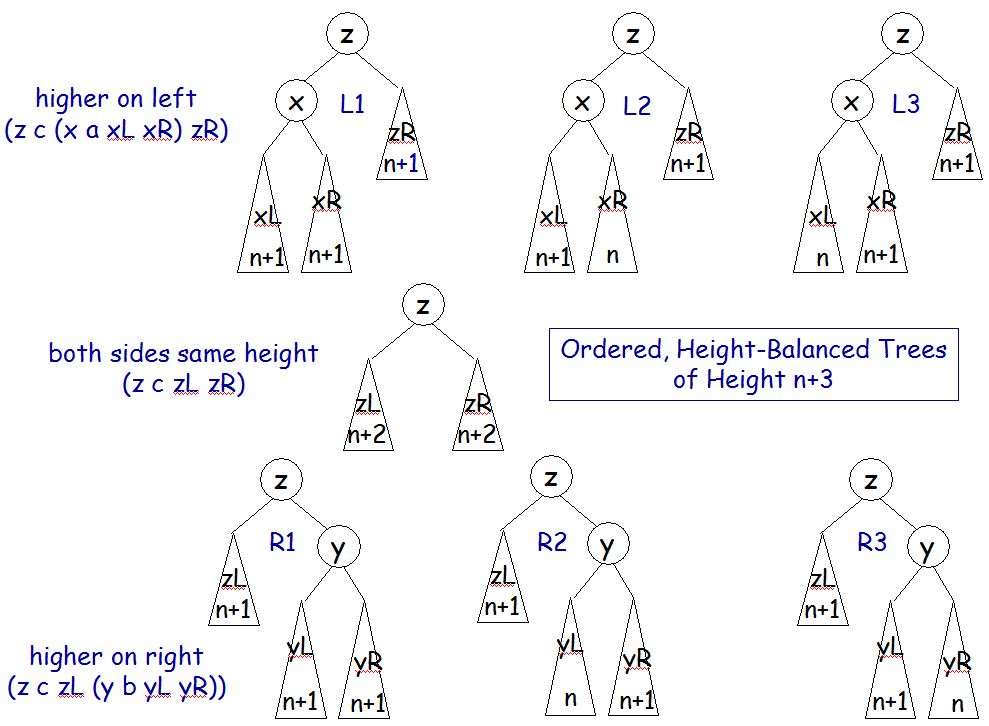
\includegraphics[scale=0.5]{images/avl-trees-ht3-or-more.png}
\end{center}
\caption{Ordered, Height-Balanced Trees of Height $n+3$}
\label{fig:trees-of-ht-n+3}
\end{figure}

\begin{ExerciseList}
\Exercise Prove
\label{thm:unbal-ht3}
theorem \{\emph{unbal-ht3}\}:
If $s$ is an unbalanced tree of height three,
then one subtree of $s$ must be empty and the the other must have height two.
That is, the following implication is a tautology. \\
((height $s$) = 3 $\wedge$ ($\neg$ (balp $s$)))
$\rightarrow$  \\
((height (lft $s$)) = 2 $\wedge$ (emptyp (rgt $s$)))
$\vee$
((emptyp (lft $s$)) $\wedge$ ((height (rgt $s$)) = 2))
\end{ExerciseList}

\section{Some Easy Cases}
The complexity of inserting a new key in a search tree
depends on where it goes, which is determined by the
relationship between its value and those of the keys
already in the tree.
Suppose, for example, we want to insert the key/data pair ($k$ $d$)
into a tree $s$ matching the tree the diagram in the middle of
Figure \ref{fig:trees-of-ht-n+3} (page \pageref{fig:trees-of-ht-n+3}).
If $k < z$, it will go into subtree \emph{zL}, and
if $k > z$, it will go into subtree \emph{zR}.
In either case, the new subtree will have height $n+2$ or $n+3$
because both \emph{zL} and \emph{zR} have height $n+2$.
So, the new tree will remain height balanced because
all of its subtrees are balanced and the heights of its
left and right subtrees will differ by one or zero.

\begin{figure}
\begin{center}
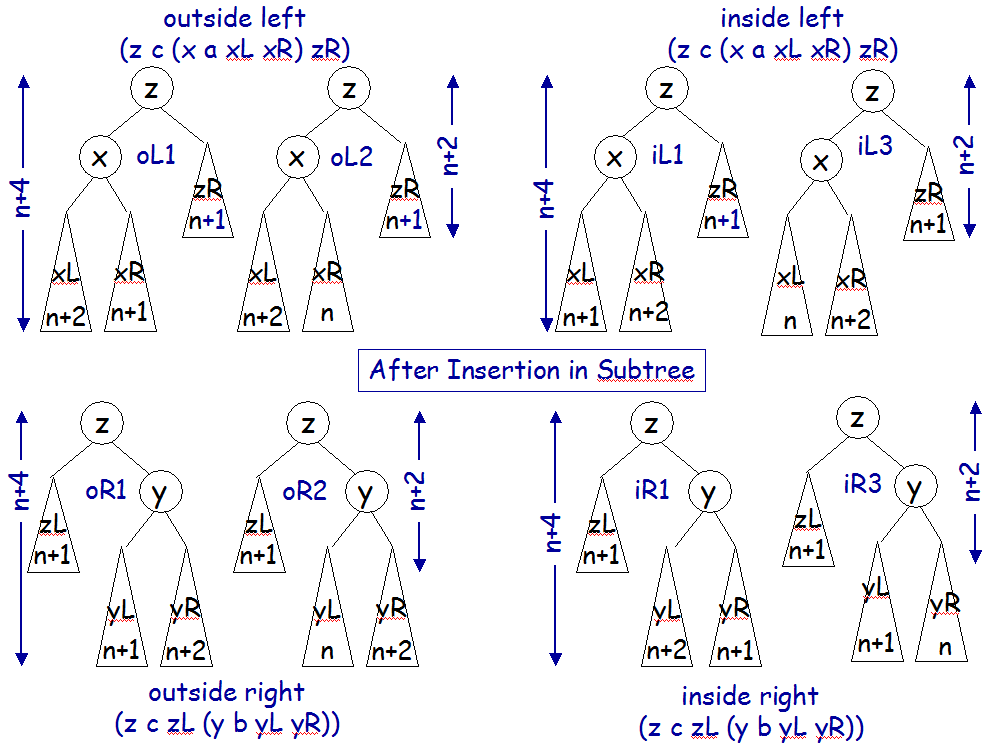
\includegraphics[scale=0.5]{images/outside-inside.png}
\end{center}
\caption{After Insertion into Tree of Height $n+3$}
\label{fig:outside-inside}
\end{figure}

Similarly, if $s$ matches the tree \emph{L1} in
Figure \ref{fig:trees-of-ht-n+3} and $k > z$,
the new key will go into subtree \emph{zR},
and the tree will remain balanced.
Likewise if $s$ matches tree \emph{L3} or \emph{L3}
and $k > z$, and there are several other cases where
the resulting tree is balanced after the insertion,
assuming $B(n)$ is true (that is, (ins ($k$ $d$) \emph{zR})
is an ordered, balanced tree with height $n+1$ or $n+2$.

The cases that need our attention are the ones where
the tree goes out of balance after the new key
is inserted into the appropriate subtree
(that is, the subtree required to keep the keys of the tree in
the proper order).
The tree will go out of balance
when the insertion into the subtree produces a taller subtree
in any of the following cases:

\label{out-of-balance-cases}
\begin{quote}
\begin{enumerate}
  \item\label{insL1xL} $k < x$: (ins ($k$ $d$) \emph{xL}) in tree \emph{L1} (Figure \ref{fig:trees-of-ht-n+3}, page \pageref{fig:trees-of-ht-n+3})
  \item\label{insL1xR} $k > x$: (ins ($k$ $d$) \emph{xR}) in tree \emph{L1}
  \item\label{insL2xL} $k < x$: (ins ($k$ $d$) \emph{xL}) in tree \emph{L2}
  \item\label{insL3xR} $k > x$: (ins ($k$ $d$) \emph{xR}) in tree \emph{L3}
  \item\label{insR1yL} $k < y$: (ins ($k$ $d$) \emph{yL}) in tree \emph{R1}
  \item\label{insR1yR} $k > y$: (ins ($k$ $d$) \emph{yR}) in tree \emph{R1}
  \item\label{insR2yR} $k > y$: (ins ($k$ $d$) \emph{yR}) in tree \emph{R2}
  \item\label{insR3yL} $k < y$: (ins ($k$ $d$) \emph{yL}) in tree \emph{R3}
\end{enumerate}
\end{quote}

Some of these cases are easier to deal with than others.
The easy ones are cases
\ref{insL1xL}, \ref{insL2xL}, \ref{insR1yR}, and \ref{insR2yR}.
In all of these cases, the tree will go out of balance after insertion
of the new item in the subtree if the insertion delivers a taller subtree.
If the tree goes out of balance, it has height $n+4$ on one side
and height $n+2$ on the other.
The factor that distinguishes these cases from the other four
is that the tall part of the tree, the part that forces it out of balance,
is a subtree on the outside boundary of the diagram,
either on the far left (cases \ref{insL1xL} and \ref{insL2xL})
or on the far right (cases \ref{insR1yR} and \ref{insR2yR}).

The other four are ``inside cases''.
That is when the tallest portion is a subtree
that is not on the outside boundary of the diagram.
Figure \ref{fig:outside-inside} (page \pageref{fig:outside-inside})
displays the status of the tree after the insertion of the new
key into a subtree in each of the cases where the tree goes out of balance.
As in Figure \ref{fig:trees-of-ht-n+3},
balanced subtrees are drawn as triangles, $x$, $y$, and $z$ are keys, etc.
The inside cases are harder to rebalance. We'll deal with them later.

Let's first look at outside-left case \ref{insL2xL} (page \pageref{insL2xL}):
the ins operator puts a new item in subtree \emph{xL} of tree \emph{L2}
(Figure \ref{fig:trees-of-ht-n+3}), producing
tree \emph{oL2}
(Figure \ref{fig:outside-inside} (page \pageref{fig:outside-inside}).
In this case, the tree is too tall on the left.
Suppose we rearrange it with key $x$ at the root
and the other subtrees placed in the spots they have to go
to keep the tree ordered.
Tree \emph{L2} Figure \ref{fig:zig-and-zag} (page \pageref{fig:zig-and-zag})
summarizes the situation before insertion,
and tree \emph{oL2} shows how it looks after insertion.
Luckily, this rearrangement rebalances the tree,
and not only for tree \emph{oL2}.
The same rearrangement works for tree \emph{oL1}
(Figure \ref{fig:outside-inside}).

\begin{figure}
\begin{center}
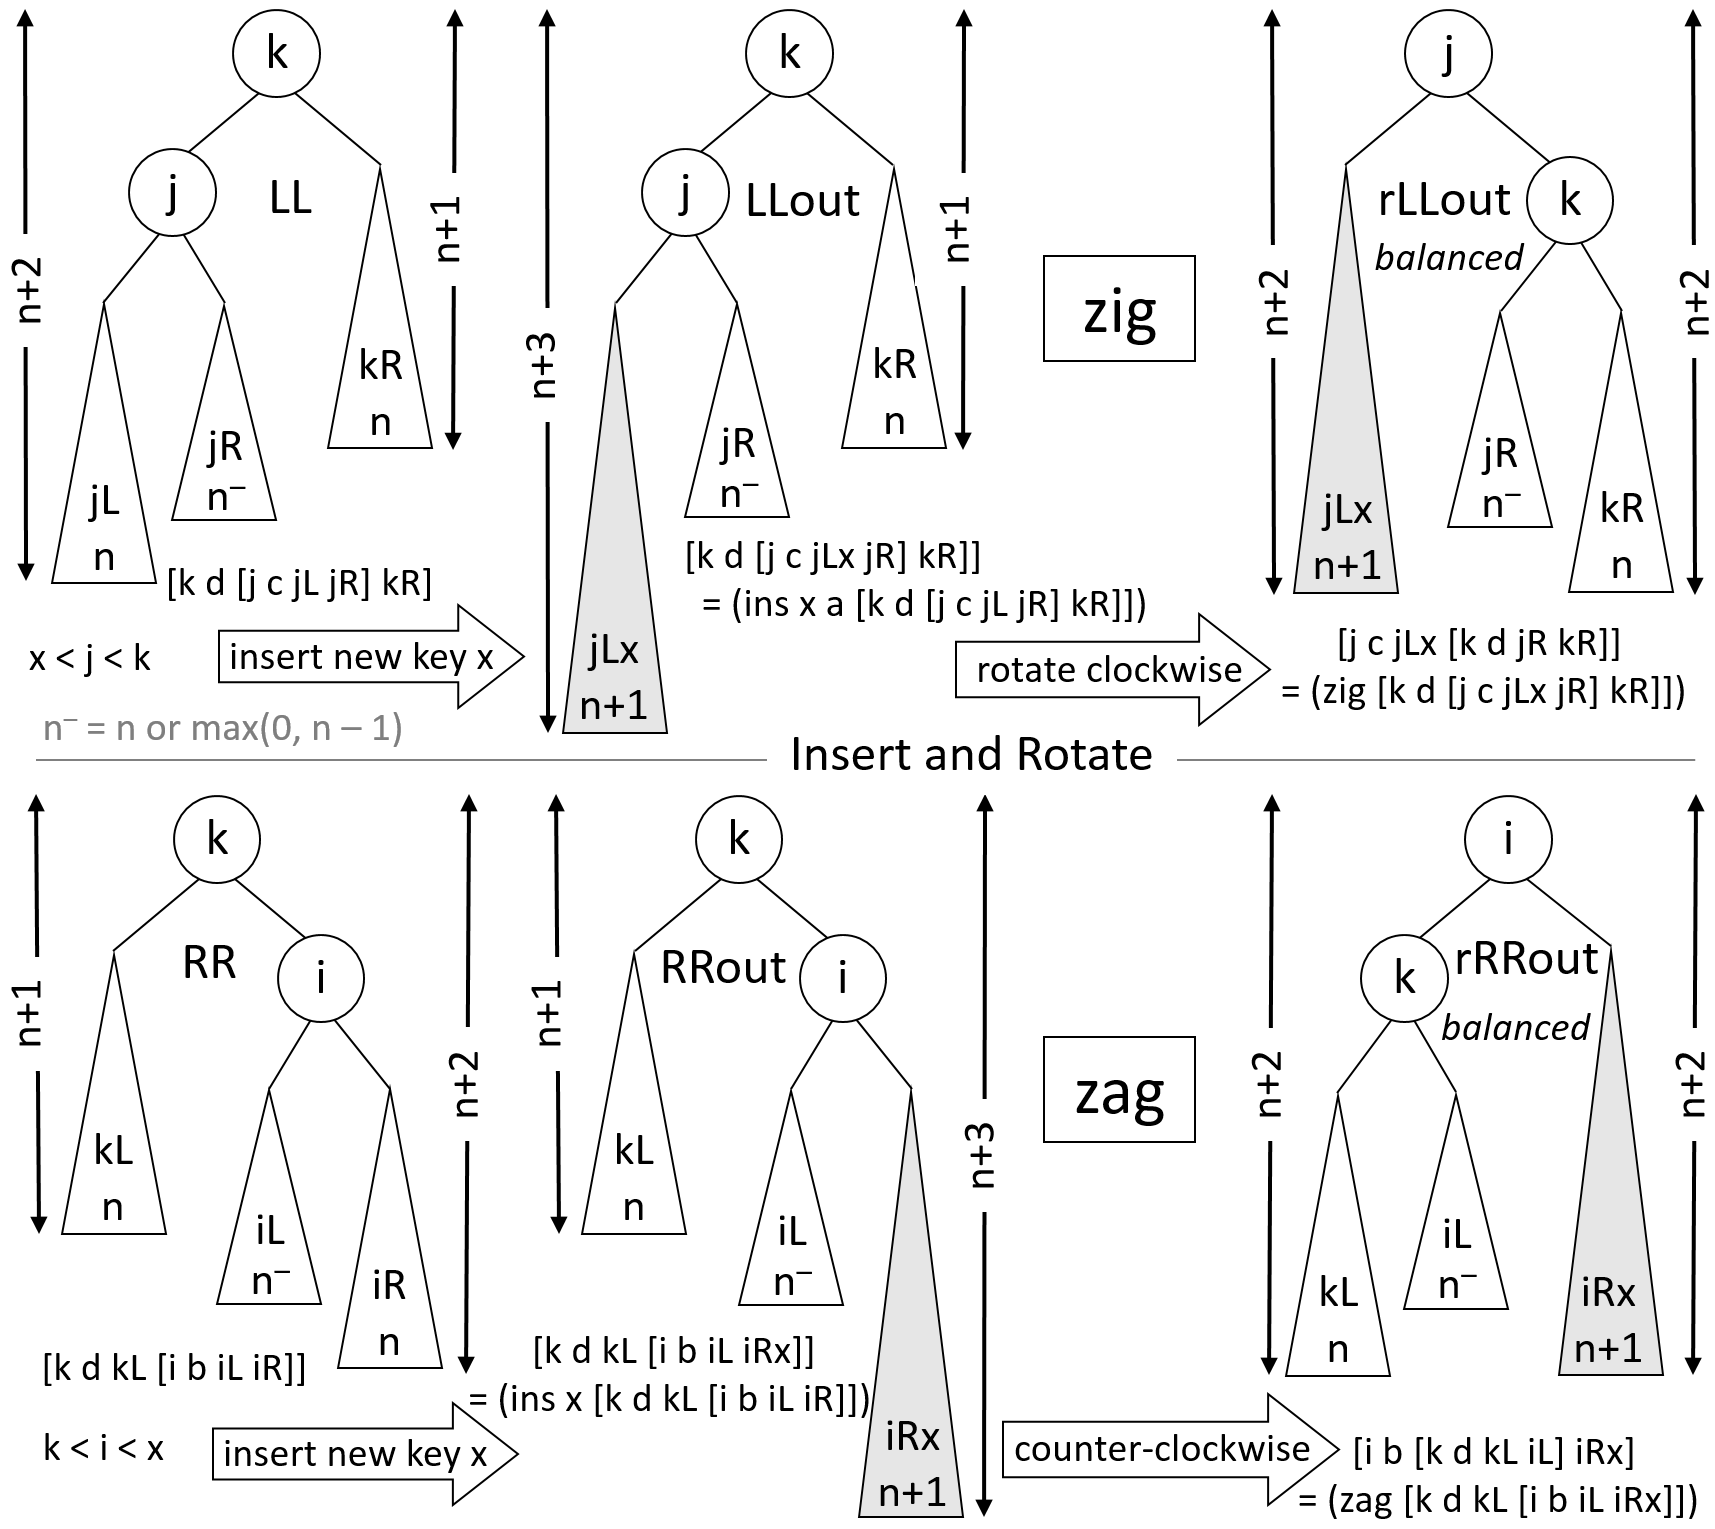
\includegraphics[scale=0.5]{images/zig-and-zag.png}
\end{center}
\caption{Insertion and Rotation, Outside Cases}
\label{fig:zig-and-zag}
\end{figure}

This type of rearrangement of an out-of-balance tree is known as a ``rotation''.
For trees \emph{oL1} and \emph{oL2}, the rotation goes clockwise.
We'll use the name ``zig'' for the operator
that performs clockwise rotations.
The operator ``zag'' will rotate in the other direction,
which is what is needed to rebalance the outside right cases.
Defining these operators in ACL2 is a matter of
converting diagrams
(Figure \ref{fig:zig-and-zag}, page \pageref{fig:zig-and-zag})
to algebraic formulas.

\label{defun:zig-and-zag}
\begin{center}
\begin{Verbatim}
(defun zig (s) ; rotate clockwise
  (let* ((z  (key s)) (c (dat s))
         (x  (key (lft s))) (a  (dat (lft s)))
         (xL (lft (lft s))) (xR (rgt (lft s)))
         (zR (rgt s)))
    (mk-tr x a xL (mk-tr z c xR zR))))
(defun zag (s) ; rotate counter-clockwise
  (let* ((z  (key s)) (c (dat s))
         (zL (lft s))
         (y  (key (rgt s))) (b  (dat (rgt s)))
         (yL (lft (rgt s))) (yR (rgt (rgt s))))
    (mk-tr y b (mk-tr z c zL yL) yR)))
\end{Verbatim}
\end{center}

To summarize, zig rebalances a tree with height $n+4$
on the ``outside left'' and height $n+2$ on the right,
but with all subtrees balanced
(Figure \ref{fig:outside-inside}, \pageref{fig:outside-inside}),
and zag rebalances trees that mirror this condition
by being too tall on the outside right.
Furthermore, all of these insertions start with a tree of height
$n+3$ and deliver a tree of the same height
(see Figure \ref{fig:zig-and-zag}, \pageref{fig:zig-and-zag}).
The induction requires the tree, after insertion, to be either
the same height as before or taller by one.
We have met that requirement,
so the proof by induction is complete for the easy cases
(cases \ref{insL1xL}, \ref{insL2xL}, \ref{insR1yR}, and \ref{insR2yR},
page \pageref{out-of-balance-cases}).

\section{Double Rotations and Insertion}

When the insertion takes place on an ``inside'' subtree
(trees \emph{iL1}, \emph{iL3}, \emph{iR1}, and \emph{iR3}
in Figure \ref{fig:outside-inside}, page \pageref{fig:outside-inside}),
it's not so easy to rebalance the tree.
Consider tree \emph{iL3}, for example.
It looks like it needs a clockwise rotation,
but zig would produce a tree with a left subtree of height $n$
and a right subtree of height $n+3$, which is even more out
of balance than the tree we started with (\emph{iL3}).
Obviously, we need a different strategy.

\begin{figure}
\begin{center}
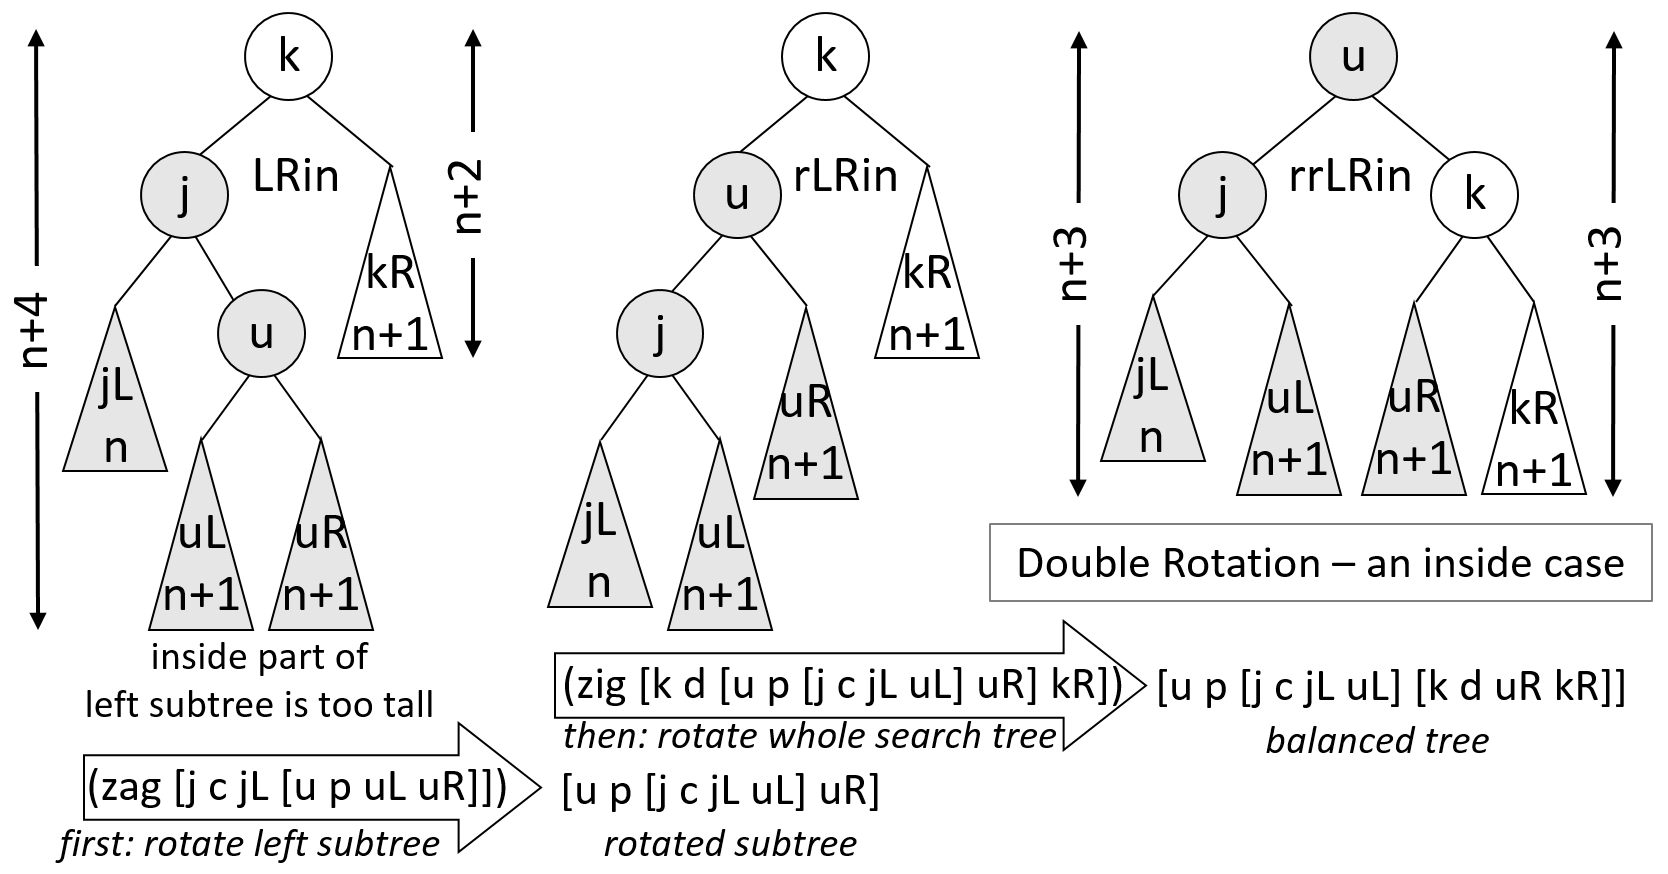
\includegraphics[scale=0.5]{images/double-rotation.png}
\end{center}
\caption{Double Rotation}
\label{fig:double-rotation}
\end{figure}

Let's stick with tree \emph{iL3}
(Figure \ref{fig:outside-inside}) to get our bearings.
Subtree \emph{xR} of tree \emph{iL3} is a balanced tree of height $n+2$.
That means it cannot be empty.
Consequently, it is possible to apply zag, the counterclockwise rotation
to the tree [\emph{x} \emph{a} \emph{xL} \emph{xR}].
It's a counterintuitive move, might not help, might even make things worse,
but it's possible, nonetheless.
\label{no-zag}(Note: It would not be possible to apply zag if \emph{xR} were empty.)

To see what happens if we apply zag to xR,
let's conjure up some names for the parts of \emph{xR}:
$u$ for (key \emph{xR}), $p$ for (key \emph{xR}),
\emph{uL} and \emph{uR} for the left and right subtrees of \emph{xR},
and $n_L$ and $n_R$ for the heights of \emph{uL} and \emph{uR}
(see Figure \ref{fig:double-rotation}, page \pageref{fig:double-rotation}).
Then,
(zag \emph{xR}) =
(zag [$x$ $a$ \emph{xL} [$u$ $p$ \emph{uL} \emph{uR}]]) =
[$u$ $p$ [$x$ $s$ \emph{xL} \emph{uL}] \emph{uR}].

At this point, we have a tree with key $z$ at the root
and a left subtree that is not empty.
This is the tree labeled \emph{zL3} Figure \ref{fig:double-rotation} (page \pageref{fig:double-rotation}).
We can use the zig operator to rotate \emph{zL3} clockwise,
producing the tree \emph{rL3} in Figure \ref{fig:double-rotation}).

Is \emph{rL3} balanced? That depends on the values of $n_L$ and $n_R$.
Fortunately, we know how these heights are constrained.
First, observe that $n+2$ = (height \emph{xR}) =
(height [$u$ $p$ \emph{uL} \emph{uR}]) = (max $n_L$ $n_R$) + 1,
so (max $n_L$ $n_R$) = $n+1$.
Furthermore, (min $n_L$ $n_R$)
is either $n$ or $n+1$, since \emph{xR} is balanced.
That ensures that at least one of the heights $n_L$ and $n_R$ must be $n+1$.
The other will be either $n$ or $n+1$.

These constraints on $n_L$ and $n_R$ guarantee
that the left and right subtrees of \emph{rL3}
(Figure \ref{fig:double-rotation}) are balanced.
In addition, the height of the left subtree of \emph{rL3}
is either $n+1$ or $n+2$,
depending on whether $n_L$ is $n$ or $n+1$,
and the height of the right subtree is $n+2$.
That means \emph{rL3} is balanced and has height $n+3$,
which completes the induction for \emph{iL3}
(case \ref{insL3xR}, page \pageref{out-of-balance-cases}).

This trick is a double rotation, first a counter-clockwise rotation (zag)
on a subtree, then a clockwise rotation (zig) on the tree as a whole.
Exactly the same double rotation works for
case \ref{insL1xR} (page \pageref{out-of-balance-cases}),
which is the other inside-left case
(tree \emph{iL1}, Figure \ref{fig:outside-inside}, page \pageref{fig:outside-inside}).

A mirror reflection of this double rotation rebalances
the inside-right cases:
case \ref{insR1yL} (page \pageref{out-of-balance-cases})
rotating tree \emph{iR1} (Figure \ref{fig:outside-inside})
and
case \ref{insR3yL} (page \pageref{out-of-balance-cases})
rotating tree \emph{iR3} (Figure \ref{fig:outside-inside}).

There are no other cases in which insertion
can cause the tree to go out of balance,
so the induction is complete.
We have, at long last, proved that $B(n)$ $\rightarrow$ $B(n+1)$ is true.
To complete the proof by induction of $\forall n.B(n)$,
we need to verify $B(0)$.
We would then know that
the operator ins
inserts a new item into an ordered, height balanced tree
of height two or more and
delivers an ordered, height-balanced tree of the same height
or at most one taller than what we started with.
Then, we would be left with a few small cases to clean up,
namely that insertion works properly on trees of height zero, one, and two.
We are going to leave these proofs to the exercises.

Expressing these ideas in terms of ACL2, rather than the
diagrams in used the proof of $B(n)$ $\rightarrow$ $B(n+1)$,
is a matter of converting the diagramed rotations to algebraic formulas,
the applying them to define the insertion operator, ins.
The function rot-R, defined as follows, performs a clockwise
rotation to rebalance a tree with a left subtree whose height is two more
than that of its right subtree, assuming that all of the subtrees are balanced.
If the left subtree is the same height as the right subtree,
or possibly taller by one, rot-R does nothing because the tree is already in balance.
The counter-clockwise rotation, rot-L, is the mirror reflection of rot-R.

With rot-R and rot-L in place, an inductive definition of the insertion
operator, ins, simply makes sure the insertion is performed in the proper
subtree to maintain order.
Of course, the new item goes into the left subtree
if the new key is smaller than the key
at the root, and into the right subtree if it's greater.
If the new key is the same as the one at the root,
we simply replace the data at the root with the new data
supplied for the insertion.
We could have made other choices in the case of equal keys,
but this choice insures that the new tree contains
the data supplied for the insertion.

\begin{center}
\label{rot-R-defun}
\begin{Verbatim}
(defun rot-R (s)     ; rebalance clockwise if ht +2 left
  (let* ((z  (key s)) (c  (dat s))          ;NOTE: s is not empty
         (zL (lft s)) (zR (rgt s)))
    (if (> (height zL) (+ (height zR) 1))           ; unbalanced?
        (if (< (height (lft zL)) (height (rgt zL))) ; inside lft?
            (zig(mk-tr z c (zag zL) zR))            ; dbl rotate
            (zig s))                                ; sngl rotate
        s)))                                        ; no rotate
(defun ins (kd s)
  (if (emptyp s)
      (mk-tr (first kd) (second kd) nil nil)      ; one-node tree
      (let* ((k (first kd)) (d (second kd))
             (z  (key s)) (c  (dat s))
             (zL (lft s)) (zR (rgt s)))
        (if (< k z)
            (rot-R (mk-tr z c (ins kd zL) zR))    ; insert left
            (if (> k z)
                (rot-L (mk-tr z c zL (ins kd zR))); insert right
                (mk-tr z d zL zR))))))            ; new root data
\end{Verbatim}
\end{center}

To make search trees really useful, we need to be able to delete items
as well as insert them.
Deletion is a little more complicated than
insertion, but uses the same basic rotation operators.
You know enough, now, to explore that idea on your own.
Check it out on Wikipedia.

\begin{ExerciseList}
\Exercise A comment on page \pageref{no-zag} points out
that is it not possible to apply the zag operator to
a tree whose right subtree is empty.
Similarly, zig does not apply to a tree whose left subtree is empty.
Explain why.

\Exercise Prove $B(0)$ (see page \pageref{ins-induction-predicate} for a defintion of $B(n)$).

\Exercise Prove that (ins $k$ $d$ nil) works properly.

\Exercise Prove that (ins $k$ $d$ $s$) works properly when (height $s$) = 1.

\Exercise Define rot-L \label{rot-L-defun}
(see the definition of rot-R, page \pageref{rot-R-defun}).

\end{ExerciseList}

\section{Fast Insertion}

The rotation operators, rot-L and rot-R, need to know the heights of subtrees
to decide whether a rotation is needed and if so, whether it should
be a single rotation or a double rotation.
Computing the height of a tree takes time because it requires counting
all the way to the leaves on every branch.
To do this, all of the nodes must be examined, so the number of steps in
the computation is proportional to the number of nodes in the tree.
Since ins has to check for possible rotations at every level in the
tree, there are a lot of height computations to perform, and this
makes the insertion process take a lot of computation steps.

Fortunately, there is a way to avoid the height computation
by recording tree height in the tree itself,
along with keys, data, and subtrees.
When a new tree is formed from a key, data, and two subtrees,
its height can be recorded quickly by extracting the heights of the
subtrees and adding one to the larger of those heights.
We use the term ``extracting'' instead of ``computing''
because the height of a subtree is right there with its key.
Extracting the height is a non-inductive operation,
like extracting the key.

The definitions of ins and the rotations stay the same as before.
The functions for tree construction and height
need to be modified to use recorded height instead of computed height.
Below are the new definitions of these functions.

\begin{center}
\begin{Verbatim}
(defun height (s) ; tree height
  (if (emptyp s)
      0           ; ht0
      (fifth s))) ; ht1
(defun mk-tr (k d lf rt)
  (list k d lf rt (+ 1 (max (height lf) (height rt)))))
\end{Verbatim}
\end{center}

In addition, the function treep, which distinguishes
trees from other kinds of things,
needs one minor modification. Instead of checking for a four-element
list, it must check for a five-element list, since the representation
of a tree now includes the height as an additional element.

The new definitions are no more complicated than the originals,
but they make a huge difference in the speed of insertion.
The number of computation steps required to insert a new
element with the original definitions is proportional to
the number of items already in the tree.
Recording heights directly in the tree,
rather than computing the height of the tree,
reduce the number of computation
steps for insertion to something proportional to the logarithm of
the number of items already in the tree.

To get a feeling for the difference, run the function measure-time,
defined below, for larger and larger trees, and measure the time
it takes. Start with, say 100 elements, then 200, 400, 800, and
so on, doubling the size of the tree each time.
Chart the number of elements and the time it takes to build the tree.
One way to do measure the time is to count the number of times
the Dracula cursor flashes between the time you enter the
(measure-time $n$) formula and the time it delivers the result.

\begin{center}
\begin{Verbatim}
(defun tree-for-timing (n)
  (if (zp n)
      nil
      (ins (list n nil) (tree-for-timing (- n 1)))))
(defun measure-time (n)
  (height (tree-for-timing n)))
\end{Verbatim}
\end{center}

\begin{aside}
The reason the function run-to-measure-time delivers only the height
of the tree it builds, rather than the tree itself, is
because it would take a lot of time and space to print the tree.
We're just interested in the amount of time it takes,
not the tree itself.
We don't have a way to deliver the computation time, directly,
so we just write a formula that will cause the computation to take place.
Then, we measure the amount of time the computer takes to do it.

Incidentally, the height of the tree
that (tree-for-timing $n$) delivers should be
$\lceil log_2(n+1) \rceil$. If it's not, something is wrong.
In other words, the following function should always deliver
the value true.

\begin{center}
\begin{Verbatim}
(defun height-right (n)
  (let* ((h     (height (tree-for-timing n)))
         (2^h   (expt 2 h))
         (2^h/2 (/ 2^h 2)))
    (and (<  2^h/2 (+ n 1))
         (<= (+ n 1) 2^h))))
\end{Verbatim}
\end{center}

\caption{Timing Tricks}
\label{timing-tricks}
\end{aside}

Then, change the mk-tr and height definitions from the ones
that record height to the original ones that compute height.
Do the timings again.
You will see that the time required by the original functions
soon gets unacceptably long.
Inserting items one by one, starting from an empty tree,
to build a tree with $n$ items takes time proportional to $n log(n)$
with recorded height.
With computed height, it takes time proportional to $n^2$.

We refer to the faster algorithm as an $n log(n)$ algorithm
and the slow one as an $n$-squared algorithm.
These are the kinds of differences in speed that turn
software that isn't practical to use
into software that is practical.
Computer scientists expend a lot of intellectual effort
figuring out how to design ways to do things that lead
to performance improvements like this.

\begin{ExerciseList}
\Exercise Carry out the timing experiment described at
the end of this section and report the results.
\end{ExerciseList}


%%% Local Variables:
%%% mode: latex
%%% TeX-master: "book"
%%% End:
